\documentclass[sigconf,authorversion,nonacm]{acmart}

%% \BibTeX command to typeset BibTeX logo in the docs
\AtBeginDocument{% \providecommand\BibTeX{{% \normalfont B\kern-0.5em{\scshape i\kern-0.25em b}\kern-0.8em\TeX}}}


    \begin{document} \title{Clustering} \author{Jake Norton} \affiliation{ \institution{University of Otago}
    \city{Dunedin} \state{Otago} \country{New Zealand} } \email{norja159@student.otago.ac.nz}


%%
%% The abstract is a short summary of the work to be presented in the
%% article.
    \begin{abstract} 
    This paper explores advanced retrieval techniques aimed at enhancing the efficiency and
    effectiveness of information retrieval systems through innovative use of graph-based and latent
    feature methodologies. We analyze three distinct approaches: Latent Approximate Document
    Retrieval (LADR), which utilizes latent features to optimize document retrieval; adaptive
    re-ranking with a corpus graph (Gar), which dynamically adjusts document rankings within a
    corpus graph to improve relevance; and adhoc retrieval through traversal of a query-document
    graph, which employs direct traversal methods to optimize query-specific document retrieval.
    \end{abstract}


%%
%% The code below is generated by the tool at http://dl.acm.org/ccs.cfm.
%% Please copy and paste the code instead of the example below.
\begin{CCSXML}
<ccs2012>
   <concept>
       <concept_id>10002951.10003317.10003338.10010403</concept_id>
       <concept_desc>Information systems~Novelty in information retrieval</concept_desc>
       <concept_significance>500</concept_significance>
       </concept>
 </ccs2012>
\end{CCSXML}

\ccsdesc[500]{Information systems~Novelty in information retrieval}

% %% Keywords. The author(s) should pick words that accurately describe %% the work being presented. Separate the
% keywords with commas.
\keywords{dense retrieval, approximate k nearest neighbour, adaptive re-ranking, neural re-ranking,
clustering hypothesis}

%%
%% This command processes the author and affiliation and title
%% information and builds the first part of the formatted document.
\maketitle
%% Make note of how the papers are related to one another
\section{Introduction} Clustering involves partitioning some set, e.g. a document collection, into a set of clusters. In
information retrieval, clustering can help to "guide retrieval"\cite{Yuan2022}. We should find that similar documents
appear in the same clusters. If a document is relevant to some query, then clearly we would expect the other documents
in said cluster to also be relevant to the given query. It is with this concept that we can see the possible benefits of
employing clustering in this field.

But, a more pertinent question is: how can we measure the effectiveness of clustering? We need to have more robust
measures for evaluating clusters. This will also be useful in determining how effective clustering really is, and how we
can improve upon it. These ideas are some of the main motivations for the three research papers discussed in this text.
In fact, it was in the pursuit of finding a reasonable way to measure the similarity of two clusterings that these
papers were intially found. 

In the first paper, Measurement of clustering effectiveness for document collections\cite{Yuan2022}, we see an
investigation into some different techniques for measuring the effectiveness of clustering. The second paper, Document
Clustering vs Topic Models: A Case Study\cite{Yuan2021}, explores two approaches to characterising document collections.
In particular, they compare the performance of clustering and topic modelling as description tools on the WSJ collection
as a case study. Finally, the third paper, Comparing Two Clusterings Using Matchings between Clusters of
Clusters\cite{Cazals2019}, is a mathematical exploration of clustering. Notably, we see the introduction of the
D-family-matching problem on intersection graphs of two clusterings. \section{Measurement of clustering effectiveness
for document collections} \subsection{Research Question} We begin with an exploration into the effectiveness of
clustering. Specifically, this paper poses the question: how might we go about measuring the effectiveness of clustering
for document collections? \subsection{Main Contributions} There are two main contributions provided in this paper; they
examine the use of extrinsic techniques in cluster evaluation, and they examine, in the context of information
retrieval, the extent of effectiveness of the standard methods of clustering.

The use of extrinsic techniques is not foreign to information retrieval. The idea of using human judgements on whether
or not certain documents are related to certain queries is well known. It is whether these techniques can be useful in
the evaluation of clusters that is uncertain. If, through the use of such techniques, we know that the documents that
are clustered together are, in fact, relevant to one another, then we can find some indication as to the quality of the
clustering. Not only did this paper find that such extrinsic techniques were useful in cluster evaluation, but that the
need for human judgement at all is unnecessary; the results obtained were sufficiently similar to those based on the
documents from retrieval systems.

The indication that results from retrieval systems may be as useful as human judgement is promising - as human labelled
data is much more difficult to obtain. In the paper, there are four measures introduced that will allow us to observe
this discovery, where $p$ is a proportion indicating the coverage of documents amongst the clusters. \begin{displaymath}
    R_c@p = \frac{\text{min number of clusters to cover }p\%\text{ of the relevant docs}}{\text{total number of
    clusters}} \end{displaymath} \begin{displaymath} R_v@p = \frac{\text{min total size of clusters to cover }p\%\text{
    of the relevant docs}}{\text{total number of docs in those clusters}} \end{displaymath} \begin{displaymath} F_c@p =
    \frac{\text{min number of clusters to cover }p\%\text{ of the retrieved docs}}{\text{total number of clusters}}
    \end{displaymath} \begin{displaymath} F_v@p = \frac{\text{min total size of clusters to cover }p\%\text{ of the
retrieved docs}}{\text{total number of docs in those clusters}} \end{displaymath} For an easier comparison of these
results, the gain is reported. That is, an estimate of the natural floor is used as a baseline, and the improvement/gain
is then observed between a given clustering and the random partitioning. 

The experiment discussed in this paper is, essentially, taking some clustering techniques of various quality, applying
said techniques to various datasets, and observing the results of the measures. An example of such results is given in
figure (1), in which we see the gain reported for the aforementioned measures on the four datasets used in the paper.
\begin{figure}[] \centering 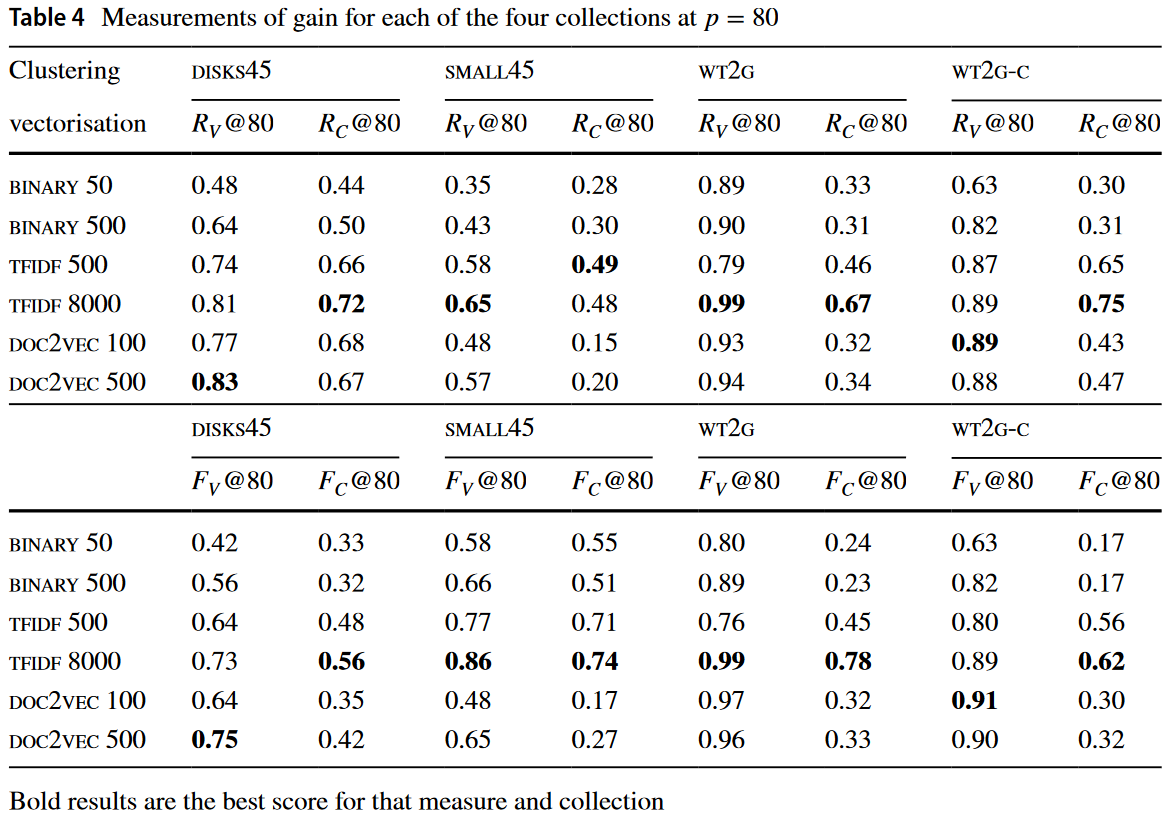
\includegraphics[width=\linewidth]{gain.png} \caption{Gain values for $p=80$ on four
collections, via \cite{Yuan2022}} \end{figure} We notice that although there are some differences between the $R$ and
$F$ measures (which the paper explains further), there are clear similarities in the results. The most prominent
similarity being the general agreement in which vectorisation method provided the best score.

As for the effectiveness of standard clustering methods, it was found that the clusterings were generally meaningful;
the clustering is "grouping documents together in a way that is consistent with their contents"\cite{Yuan2022}. However,
it is not yet clear if this is entirely useful to information retrieval. We also note that it appears as though the
quality of a clustering may decrease with an increase in the size of the collection. It may be worth looking into this
further, especially given the scale often encountered in information retrieval. \section{Document Clustering vs Topic
Models: A Case Study} \subsection{Topic Modelling} As a brief aside, we shall highlight topic modelling - in which we
take each topic to be a mapping from the set of terms in our collection to a set of weights. The words which are highly
weighted for a topic should be representative of some semantic theme. \subsection{Research Question} Here, we present a
case study comparing clustering and topic modelling as description tools for the WSJ document collection. This
comparison being the main driving force behind the paper. \subsection{Main Contributions} The main contributions for
this paper are as follows: two simple cluster labelling methods are compared, significant alignment between the clusters
and topic labels on the WSJ collection is found, and said topic-cluster alignment is used to show that words/documents
close to the centroid are not good representations of the clusters.

For their first contribution, they highlight two basic methods for labelling clusters: the central keywords method, and
the cluster keywords method. In central keywords, we select the N highest-weighted words from only the documents close
to the centroids. For cluster keywords, we again select the N highest-weighted words - but from amongst all the
documents in the cluster. It is clear that these methods are similar in nature and name, and it is unfortunate that more
care was not taken to differentiate the two. Some areas of the text require further clarification, for example, in the
conclusion there is a description of what appears to be the central keywords method as being "highly
effective"\cite{Yuan2021}, and yet elsewhere there are plentiful remarks that this method is a "complete
failure"\cite{Yuan2021}, and that the cluster keywords method was found to be more reliable. Nonetheless, it is easily
observed in table (1) that the cluster keywords and topic labels share many more similarities than the central keywords.
\begin{table}[] \begin{tabular}{lp{5cm}} \hline Cluster terms & quarter, cent, net, share, earn, loss, sale, revenu,
profit, incom \\ \hline Topic terms  & quarter, cent, share, net, earn, loss, sale, profit, revenu, incom\\ \hline
Centre terms & laser, pnc, hansen, doctrin, billion, mile, mercer, quarter, daughter, court\\ \hline \end{tabular}
\caption{An example of keywords and topic labels, via Table 3a \cite{Yuan2021}} \end{table} Further, it was found that
there is significant alignment between the clusters and the topic labels, at least for the corpus in question. This
paper found this result surprising, since clustering and topic modelling are rather different approaches. It would be
very interesting to see these results replicated with other collections, or for this discovery to be more generalised.

The topic-cluster alignment was also used to demonstrate the unsuitability of choosing words/documents close to the
centroid as a representative of the cluster as a whole. It seems perfectly logical to assume that an item close to a
centroid would be a good representative of the cluster. However,  likely due to the nature of working in higher
dimensions, this was not found to be the case - or at least, it was not found to be true for the collection in question.
\section{Comparing Two Clusterings Using Matchings between Clusters of Clusters} \subsection{Research Questions} In this
paper, we take a step away from information retrieval and consider clustering in a more theoretical sense. The most
prominent question lies in the exploration of the relationship between two clusterings, and how we might define this.
But another question posed is in regards to the scale at which cluster might merge. \subsection{Main Contributions}
There are a plethora of contributions provided in this paper, all very mathematical in nature. We shall briefly outline
what these are, and then focus on the more interesting results. A new combinatorial optimisation problem,
D-Family-Matching, is introduced - and then proven to be very difficult (NP-complete and APX-hard). The paper describes
some efficient algorithms for general graphs, and then shows these algorithms are capable of identifying meta-clusters
(clusters of clusters) between a given clustering and an edited version. Finally, they provide some insights into the
scale at which clusters combine.

The problem of D-Family-Matching introduced in this paper is very interesting. From two clusterings, $F$ and $F'$, we
obtain the intersection graph G. We take a node of $G$ to represent a cluster, with an edge between two such nodes
indicating that the intersection between said clusters is nonempty - or rather, that there is at least one element
shared between them. In fact, the weight of an edge is the number of elements common to both clusters. The idea of this
problem is to find "an explicit many-to-many correspondence between groups of clusters of the two
clusterings"\cite{Cazals2019}. The parameter $D$ being an upper bound of the diameter of the graph G.

Let us now consider a reasonably straightforward example from the paper, using a 2D dataset of 40 points.
\begin{figure}[H] \centering 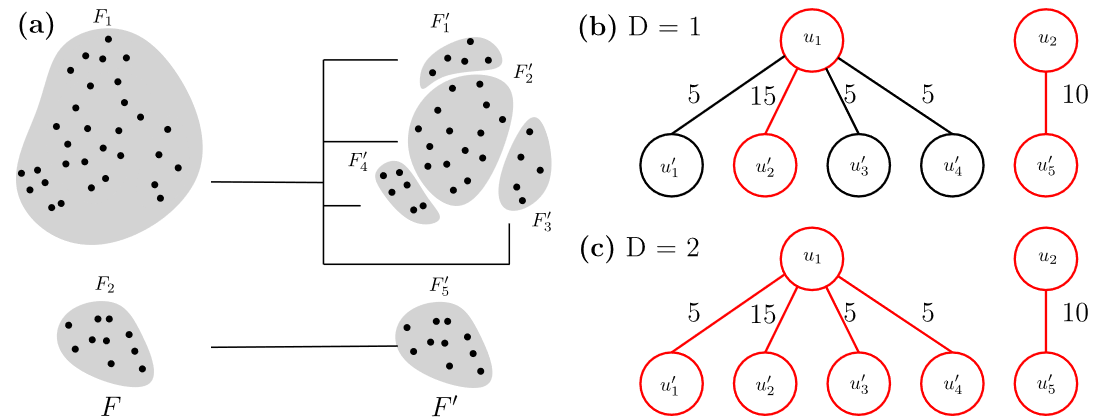
\includegraphics[width=\linewidth]{dfamilymatching.png} \caption{Example of
D-Family-Matching, via \cite{Cazals2019}} \end{figure} In (a) we see the two different clusterings $F$ and $F'$ of the
dataset, with the D-Family-Matching graphs for $D=1$ and $D=2$ showcased in (b) and (c) respectively. In the case of
$D=1$ (1-to-1), we only match the clusters with the highest weights - this is the method most existing methods use. With
$D=2$, we are now able to match $F_1$ to the meta-cluster $\{F'_1, F'_2, F'_3, F'_4\}$ - this is the 1-to-many case.

If we now look beyond the example in figure (2), we may wonder what $D>2$ might represent. For such values, we observe
the many-to-many cases. These deal with the case where we have different clusters from each clustering corresponding to
each other without a "good" matching. We can think of $D$ as being indicative of the complexity of the involved
meta-clusters.

This is all very exciting, but may it be unclear as to how this relates to the other papers discussed, or to information
retrieval at all. In fact this approach to clustering, and the introduction of the variable $D$, may bring us closer to
figuring out how to appropriately choose the number of clusters. Further exploration of their works, perhaps with a
particular focus on information retrieval, would prove very interesting. \section{Relations between the papers} It is
immediately obvious that all three papers chosen are primarily focus on clustering; it is the main link between them.
Further than this though, it is the exploration of evaluation that truly ties these papers together.

In \cite{Yuan2022} and \cite{Cazals2019}, we see an exploration into the evaluation of clustering. The former primarily
focuses on the effectiveness of certain techniques for cluster evaluation, whereas the latter delves more into the
relationship between two clusterings. In both papers, it is clear that there is an investigation into the evaluation of
clustering.

As for \cite{Yuan2021}, there are more similarities held to \cite{Yuan2022} than to \cite{Cazals2019}. Ignoring the
obvious connection of the papers sharing the same group of authors, we see that they share the focus of clustering in
the context of information retrieval - particularly looking at the clustering of documents. To motivate advancements of
one field, e.g. information retrieval, it is important to consider related advancements that originate elsewhere. It is
with this idea that we may consider \cite{Cazals2019} as being a suitable selection.

The link between \cite{Yuan2021} and \cite{Cazals2019}, then, is very much the weakest. It is with the inclusion of the
other paper that we are truly able see to much of a link at all - besides, of course, the central theme of clustering.
\section{Is there a unique ideal clustering?} If we revisit figure (2), we observe that for the same set of data we have
two different clusterings. This inspires the question: is there a unique ideal clustering? Further, is there some ideal
number of clusters? Or perhaps an ideal partitioning of a given set? There are many more such questions that come to
mind.

For individual collections, there must be some unique clustering that best suits the desired task. How might we find
this, and what would we consider to be "best"? In a more general sense, is it possible to find an ideal number of
clusters?

Using the results regarding cluster comparison and evaluation, we should be able to determine if a given clustering of
an specific collection is the "best" such clustering. The knowledge of the collection will allow us to have some notion
of "best" for the given context. However, the more difficult question remains: how can we reliably find this clustering?

In fact, \cite{Yuan2022} and \cite{Cazals2019} both touch on this question. With \cite{Cazals2019} in particular
assessing their parameter $D$ and its implications for choosing the "correct" number of clusters. Although we neglected
to touch on the concept in this text, the notion of cluster stability is also investigated by both of these papers. This
could also be beneficial in the answering of our question.

Perhaps, then, clustering could benefit from a proper investigation into the choice in the number of clusters. Such an
investigation could begin with a thorough review of existing methods and techniques for partitioning some dataset into
clusters. Then, we could examine the effects of cluster sizes, and the number of clusters, possibly even incorporating
this notion of $D$. This exploration would be based in the context of information retrieval, but would clearly have
implications for clustering as a whole. \section{Can morphological techniques improve clustering?} If we, again, assume
that we can reliably evaluate our clusters and clusterings, might there be a way we can improve upon them? Specifically,
could morphological techniques such as stemming improve the quality of the clustering? Further, how would this effect
any meaning potentially held within the clustering?

To investigate this, this author proposes that we begin by exploring the effects of said morphological techniques on
some clusterings of a well-known corpus. The results of this should give some indication as to whether such a proposal
is at all useful. It will also allow us to more closely examine the nature of the clusters themselves, perhaps shedding
some light on what meaning these clusters hold. \section{Conclusion} Clustering has much room for further investigation.
At first glance it may seem like a simple problem (grouping things together), but as we have seen, even evaluating a set
of clusters can be very complex. It is a very interesting field of study, and one that could benefit from further
research.

In \cite{Yuan2022}, we saw an examination of different techniques for measuring the effectiveness of clustering, as well
as an exploration into the suitability of standard clustering methods for information retrieval. From this we have
discovered several measures that can be used to evaluate a clustering (in the context of information retrieval). Another
result of note was the indication that the quality of a clustering may decrease as the size of the collection increases.

\cite{Yuan2021} gave us a good comparison of document clustering and topic modelling. In particular, we got to explore
clustering as a descriptive tool - and we saw the unsuitability of using items close to the centroid as a representative
of a cluster.

Finally, in \cite{Cazals2019}, we were introduced to the D-Family-Matching problem. This paper holds some very exciting
results, and it would be very interesting to see them applied to information retrieval. \section*{}
%% The next two lines define the bibliography style to be used, and
%% the bibliography file.
\bibliographystyle{ACM-Reference-Format} \bibliography{references}

\end{document} \endinput

